\documentclass[a4paper,12pt, oneside]{book}

% \usepackage{fullpage}
\usepackage[italian]{babel}
\usepackage[utf8]{inputenc}
\usepackage{amssymb}
\usepackage{amsthm}
\usepackage{graphics}
\usepackage{amsfonts}
\usepackage{listings}
\usepackage{amsmath}
\usepackage{amstext}
\usepackage{engrec}
\usepackage{rotating}
\usepackage{verbatim}
\usepackage[safe,extra]{tipa}
% \usepackage{showkeys}
\usepackage{multirow}
\usepackage{hyperref}
\usepackage{microtype}
\usepackage{fontspec}
\usepackage{enumerate}
\usepackage{physics}
\usepackage{braket}
\usepackage{marginnote}
\usepackage{pgfplots}
\usepackage{cancel}
\usepackage{polynom}
\usepackage{booktabs}
\usepackage{enumitem}
\usepackage{framed}
\usepackage{pdfpages}
\usepackage{pgfplots}
\usepackage{algorithm}
% \usepackage{algpseudocode}
\usepackage[cache=false]{minted}
\usepackage{mathtools}
\usepackage[noend]{algpseudocode}
\newcommand*{\bfrac}[2]{\genfrac{}{}{0pt}{}{#1}{#2}}

\usepackage{tikz}\usetikzlibrary{er}\tikzset{multi  attribute /.style={attribute
    ,double  distance =1.5pt}}\tikzset{derived  attribute /.style={attribute
    ,dashed}}\tikzset{total /.style={double  distance =1.5pt}}\tikzset{every
  entity /.style={draw=orange , fill=orange!20}}\tikzset{every  attribute
  /.style={draw=MediumPurple1, fill=MediumPurple1!20}}\tikzset{every
  relationship /.style={draw=Chartreuse2,
    fill=Chartreuse2!20}}\newcommand{\key}[1]{\underline{#1}}
\usetikzlibrary{arrows.meta}
\usetikzlibrary{decorations.markings}
\usetikzlibrary{arrows,shapes,backgrounds,petri}
\tikzset{
  place/.style={
    circle,
    thick,
    draw=black,
    minimum size=6mm,
  },
  transition/.style={
    rectangle,
    thick,
    fill=black,
    minimum width=8mm,
    inner ysep=2pt
  },
  transitionv/.style={
    rectangle,
    thick,
    fill=black,
    minimum height=8mm,
    inner xsep=2pt
  }
} 
\usetikzlibrary{automata,positioning,chains,fit,shapes}
\usepackage{fancyhdr}
\pagestyle{fancy}
\fancyhead[LE,RO]{\slshape \rightmark}
\fancyhead[LO,RE]{\slshape \leftmark}
\fancyfoot[C]{\thepage}
\usepackage[usenames,dvipsnames]{pstricks}
\usepackage{epsfig}
\usepackage{pst-grad} % For gradients
\usepackage{pst-plot} % For axes
\usepackage[space]{grffile} % For spaces in paths
\usepackage{etoolbox} % For spaces in paths
\makeatletter % For spaces in paths
\patchcmd\Gread@eps{\@inputcheck#1 }{\@inputcheck"#1"\relax}{}{}
\makeatother
\usepackage{lipsum}
\DeclareSymbolFont{symbolsC}{U}{txsyc}{m}{n}
\DeclareMathSymbol{\strictif}{\mathrel}{symbolsC}{74}
\title{Computational Systems Biology}
\author{UniShare\\\\Davide Cozzi\\\href{https://t.me/dlcgold}{@dlcgold}}
\date{}

\pgfplotsset{compat=1.13}
\begin{document}
\maketitle

\definecolor{shadecolor}{gray}{0.80}
\setlist{leftmargin = 2cm}
\newtheorem{teorema}{Teorema}
\newtheorem{definizione}{Definizione}
\newtheorem{esempio}{Esempio}
\newtheorem{corollario}{Corollario}
\newtheorem{lemma}{Lemma}
\newtheorem{osservazione}{Osservazione}
\newtheorem{nota}{Nota}
\newtheorem{esercizio}{Esercizio}
\algdef{SE}[DOWHILE]{Do}{doWhile}{\algorithmicdo}[1]{\algorithmicwhile\ #1}
\tableofcontents
\renewcommand{\chaptermark}[1]{%
  \markboth{\chaptername
    \ \thechapter.\ #1}{}}
\renewcommand{\sectionmark}[1]{\markright{\thesection.\ #1}}
\newcommand{\floor}[1]{\lfloor #1 \rfloor}
\newcommand{\MYhref}[3][blue]{\href{#2}{\color{#1}{#3}}}%
\chapter{Introduzione}
\textbf{Questi appunti sono presi a lezione. Per quanto sia stata fatta
  una revisione è altamente probabile (praticamente certo) che possano
  contenere errori, sia di stampa che di vero e proprio contenuto. Per
  eventuali proposte di correzione effettuare una pull request. Link: }
\url{https://github.com/dlcgold/Appunti}.\\
\chapter{Introduzione alla modellistica}
\section{Systems Biology}
Per descrivere sistemi biologici complessi si hanno vari tipi di modelli.\\
Kitano (il ``padre'' di quest'ambito), nel 2002, disse che per capire i sistemi
biologici complessi bisogna integrare risultati sperimentali e metodi
computazionali, ottenendo quindi la 
vera e propria \textbf{Systems Biology}. Tramite l'interazione di vari
componenti si ottengono tali sistemi. Disse infatti:
\begin{center}
  \textit{To understand complex biological systems requires the integration of
    experimental and computational research — in other words a systems biology
    approach.} 
\end{center}
Weston, nel 2004, ha aggiunto l'importanza dello studio delle interazioni e
delle regolazioni tra i vari componenti del sistema, studiando le risposte alla
genetica o alle perturbazioni ambientali, al fine di capire nuove proprietà del
sistema. Infatti disse:
\begin{center}
  \textit{Systems biology is the analysis of the relationships among the
    elements in a system in response to genetic or environmental perturbations,
    with the goal of understanding the system or the emergent properties of the
    system} 
\end{center}
Ideker (altro ``padre'' di quest'ambito), già nel 2001, aveva definito la System
Biology come l'integrazione dei 
dati sperimentali con i modelli matematici che descrivono componenti e
interazioni, al fine di simulare il comportamento complessivo ``in silico''. Nel
dettaglio, citandolo:
\begin{center}
  \textit{Systems biology studies biological systems by systematically
    perturbing them (biologically, genetically, or chemically); monitoring the
    gene, protein, and informational pathway responses; integrating these data;
    and ultimately, formulating mathematical models that describe the structure
    of the system and its response to individual perturbations} 
\end{center}
Ai metodi standard della biologia quindi si aggiungono le teorie
informatiche, quelle matematiche, quelle fisiche, quelle chimiche, quelle
ingegneristiche. A partire dal fenomeno biologico quindi si effettuando
esperimenti, ottenendo dei dati sperimentali relativi alle funzioni, alle
strutture e alle interazioni delle varie componenti biologiche. A partire da
questi dati si costruisce un \textbf{modello matematico} che porterà alla
produzione 
di \textit{ipotesi} a partire da esso. Inoltre l'insieme di ipotesi produrrà
nuovi dati che potranno essere anche usati per rifinire il modello
stesso. Inoltre tali ipotesi possono portare a sperimentazioni in \textbf{dry
  lab}, quindi ``in silico'' tramite simulazioni, ma anche in \textbf{wet lab},
quindi in laboratorio qualora possibile. Tali sperimentazioni contribuiranno a
migliorare i dati stessi, producendone anche di nuovi. Si ha quindi un sistema
ciclico di costante miglioramento della ricerca stessa, come visualizzabile in
figura \ref{fig:csb}.
\begin{figure}
  \centering
  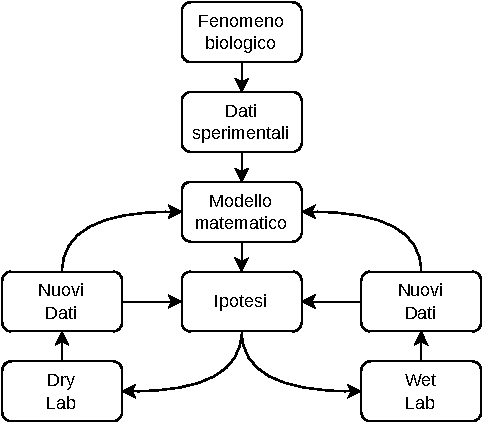
\includegraphics[scale = 0.8]{img/csb.pdf}
  \caption{Grafico rappresentante il processo ciclico della Systems Biology}
  \label{fig:csb}
\end{figure}

\end{document}

% LocalWords: 